\documentclass[12pt]{article}

% Packages
\usepackage{amsmath, amssymb, amsthm, geometry, mathrsfs, mathtools, tikz}
\usepackage[colorlinks=true, linkcolor=blue, pdfusetitle]{hyperref}

% Page Geometry
\geometry{a4paper, margin=1in}

% Theorem Environments
\renewcommand{\qedsymbol}{$\blacksquare$}
\newtheorem{problem}{Problem}

\title{3.5 Rigorous Practice Problem Set}
\author{Tashfeen Omran}
\date{\today}

\begin{document}

\maketitle

\tableofcontents
\newpage

\section{Concept Checklist \& Question Mapping}
\label{sec:checklist_start}
The following checklist cross-references the theoretical concepts and proof techniques extracted from the source material with the 30 rigorous problems generated in this document.

\begin{itemize}
    \item \textbf{Trivial Proof (Continuous Domain):} Problem 3
    \item \textbf{Vacuous Proof (Continuous Domain):} Problems 1, 7, 11, 25
    \item \textbf{Vacuous Proof (Discrete Domain):} Problems 2, 15, 21, 27
    \item \textbf{Direct Proof (Parity of Integers):} Problems 4, 10, 24
    \item \textbf{Direct Proof (Divisibility):} Problems 5, 12
    \item \textbf{Direct Proof (Rational Numbers):} Problems 6, 20
    \item \textbf{Algebraic Manipulations (Completing the Square):} Problems 1, 3, 25, 27
    \item \textbf{Algebraic Manipulations (Cyclic Symmetry):} Problem 7
    \item \textbf{Domain Boundary Conditions:} Problems 2, 21
    \item \textbf{Logical Equivalences:} Problems 8, 13, 22
    \item \textbf{Counterexamples:} Problems 9, 14, 23, 29
    \item \textbf{Fallacy Identification (Misapplying Axioms):} Problem 19
    \item \textbf{Fallacy Identification (Variable Aliasing):} Problem 28
    \item \textbf{Abstract Real-World Modeling (AI Constraint Sets):} Problem 17
    \item \textbf{Abstract Real-World Modeling (Quant Finance):} Problem 18
    \item \textbf{Abstract Real-World Modeling (Measure-Theoretic Probability):} Problem 26
    \item \textbf{Set Theory (Subset Inclusion \& Equality):} Problems 16, 29, 30
\end{itemize}

\newpage

\section{Problem Set}
\label{sec:problems}

\begin{problem}
Prove that if $x \in \mathbb{R}$ and $x^2 - 6x + 10 < 0$, then $x^3 \ge 50$.
\end{problem}

\begin{problem}
Prove that if $n \in \mathbb{N}$ and $3|n - 2| + 2|n + 1| \le 2$, then $n^2 \le 0$.
\end{problem}

\begin{problem}
Prove that if $x, y \in \mathbb{R}$, then $2x^2 + 2y^2 \ge 4xy$.
\end{problem}

\begin{problem}
Prove that if $a, b \in \mathbb{Z}$ are odd, then $5a - 3b$ is an even integer.
\end{problem}

\begin{problem}
Prove that if $a, b, c \in \mathbb{Z}$ such that $a \mid b$ and $a \mid c$, then $a \mid (4b - 7c)$.
\end{problem}

\begin{problem}
Prove that if $r, s \in \mathbb{Q}$, then $3r + 2s \in \mathbb{Q}$.
\end{problem}

\begin{problem}
Prove that if $x, y, z \in \mathbb{R}$ and $x^2 + y^2 + z^2 < xy + xz + yz$, then $x+y+z = 100$.
\end{problem}

\begin{problem}
Establish the logical equivalence of $P \implies (Q \lor R)$ and $(P \land \neg Q) \implies R$.
\end{problem}

\begin{problem}
Find a counterexample to the proposition: ``For all $x, y \in \mathbb{R}$, if $x^2 > y^2$, then $x > y$.''
\end{problem}

\begin{problem}
Prove that if $n \in \mathbb{Z}$ is even, then $n^2 + 5n + 7$ is odd.
\end{problem}

\begin{problem}
Prove that if $x \in \mathbb{R}$ and $x^4 + 2x^2 + 3 \le 0$, then $\int_0^x e^{t^2} dt = 0$.
\end{problem}

\begin{problem}
Prove that if $a, b \in \mathbb{Z}$ and $a \mid b$, then $a^3 \mid b^3$.
\end{problem}

\begin{problem}
Establish the logical equivalence of $(P \implies Q) \land (P \implies R)$ and $P \implies (Q \land R)$.
\end{problem}

\begin{problem}
Find a counterexample to the proposition: ``For all $a, b, c \in \mathbb{Z}$, if $a \mid (bc)$, then $a \mid b$ or $a \mid c$.''
\end{problem}

\begin{problem}
Prove that if $x \in \mathbb{Z}$ and $x^2 + x + 1$ is even, then $x^5$ is even.
\end{problem}

\begin{problem}
Prove that if $A, B, C$ are sets such that $A \subseteq B$ and $B \subseteq C$, then $A \subseteq C$.
\end{problem}

\begin{problem}
Derive the probability measure $\mathbb{P}(Q(X))$ for an AI fallback protocol $Q(x)$ triggered by the precondition $P(x) : \|x - \mu\|^2 + \|x - \nu\|^2 < 0$ for vectors $x, \mu, \nu \in \mathbb{R}^d$.
\end{problem}

\begin{problem}
Prove that if a quantitative finance strategy $\omega$ yields a risk-free profit with zero initial investment in an arbitrage-free market, then $\omega$ also guarantees a risk-free loss.
\end{problem}

\begin{problem}
Find the flaw in the following proof: ``Theorem: Let $x \in \mathbb{C}$. If $x^2 < 0$, then $x^4 > 0$. Proof: The square of any number is non-negative, so $x^2 < 0$ is impossible. Thus the implication is vacuously true.''
\end{problem}

\begin{problem}
Prove that if $x, y \in \mathbb{Q}$, then $x^2 + 2xy + y^2 \in \mathbb{Q}$.
\end{problem}

\begin{problem}
Prove that if $n \in \mathbb{N}$ and $n + \frac{1}{n} < 2$, then $n^3 = 10$.
\end{problem}

\begin{problem}
Establish the logical equivalence of $P \implies Q$ and $\neg Q \implies \neg P$.
\end{problem}

\begin{problem}
Find a counterexample to the proposition: ``For all $x \in \mathbb{R}$, if $x^3 > 0$, then $x > 1$.''
\end{problem}

\begin{problem}
Prove that if $a, b \in \mathbb{Z}$ are odd, then $ab$ is odd.
\end{problem}

\begin{problem}
Prove that if $x \in \mathbb{R}$ and $4x^2 - 4x + 2 \le 0$, then $x = 100$.
\end{problem}

\begin{problem}
Derive the probability measure for the event $A = \{ \omega \in \Omega : X(\omega)^2 + Y(\omega)^2 < 2X(\omega)Y(\omega) \}$ for real-valued random variables $X, Y$ under the Kolmogorov axioms.
\end{problem}

\begin{problem}
Prove that if $x \in \mathbb{Z}$ and $2x = x^2 + 2$, then $x$ is odd.
\end{problem}

\begin{problem}
Find the flaw in the following proof: ``Theorem: Let $x, y \in \mathbb{Z}$. If $x, y$ are odd, then $x-y$ is a multiple of $4$. Proof: Let $x = 2k+1$ and $y = 2k+1$. Then $x-y = (2k+1) - (2k+1) = 0 = 4(0)$.''
\end{problem}

\begin{problem}
Find a counterexample to the assertion: ``For any sets $A, B, C$, if $A \subseteq B \cup C$, then $A \subseteq B$ or $A \subseteq C$.''
\end{problem}

\begin{problem}
Prove that if $A, B$ are sets such that $A \cap B = A \cup B$, then $A = B$.
\end{problem}

\newpage

\section{Detailed Solutions}
\label{sec:solutions}

\subsection*{Solution 1}
\begin{proof}
We proceed via a vacuous proof. Let $P(x)$ be the hypothesis $x^2 - 6x + 10 < 0$. By completing the square, we rewrite the quadratic expression:
\[ x^2 - 6x + 10 = (x^2 - 6x + 9) + 1 = (x-3)^2 + 1 \]
By the axioms of real numbers, the square of any real number is non-negative, meaning $(x-3)^2 \ge 0$ for all $x \in \mathbb{R}$. Adding $1$ to both sides yields:
\[ (x-3)^2 + 1 \ge 1 > 0 \]
Thus, the statement $(x-3)^2 + 1 < 0$ is a logical contradiction. Because the hypothesis $P(x)$ is false for all $x \in \mathbb{R}$, the implication is vacuously true.
\end{proof}

\subsection*{Solution 2}
\begin{proof}
We proceed via a vacuous proof. The domain is $\mathbb{N} = \{1, 2, 3, \dots\}$. Since $n \in \mathbb{N}$, we have the rigid lower bound $n \ge 1$. Consequently, $n + 1 \ge 2$. Because absolute values preserve non-negativity and magnitude for positive numbers, $|n + 1| \ge 2$. Multiplying by $2$ yields:
\[ 2|n + 1| \ge 4 \]
Furthermore, by the definition of absolute value, $3|n - 2| \ge 0$. Adding these two inequalities together, we obtain:
\[ 3|n - 2| + 2|n + 1| \ge 0 + 4 = 4 \]
Since $4 > 2$, the hypothesis $3|n - 2| + 2|n + 1| \le 2$ is strictly false for every $n \in \mathbb{N}$. Because the hypothesis is false for all elements in the domain, the implication is vacuously true.
\end{proof}

\subsection*{Solution 3}
\begin{proof}
We proceed via a trivial proof. Let $Q(x,y)$ be the conclusion $2x^2 + 2y^2 \ge 4xy$. We evaluate $Q(x,y)$ by subtracting $4xy$ from both sides:
\[ 2x^2 - 4xy + 2y^2 \ge 0 \]
Factoring out the common scalar $2$ yields:
\[ 2(x^2 - 2xy + y^2) \ge 0 \]
Recognizing the perfect square, we rewrite the expression as:
\[ 2(x-y)^2 \ge 0 \]
By the properties of real numbers, $(x-y)^2 \ge 0$ for all $x, y \in \mathbb{R}$. Multiplying by $2$ preserves the inequality, so $2(x-y)^2 \ge 0$ is universally true. Because the conclusion is always true over the domain, the implication is trivially true.
\end{proof}

\subsection*{Solution 4}
\begin{proof}
We proceed via a direct proof. Assume $a$ and $b$ are odd integers. By the definition of odd integers, there exist integers $k, m \in \mathbb{Z}$ such that $a = 2k + 1$ and $b = 2m + 1$. We substitute these expressions into the polynomial $5a - 3b$:
\begin{align*}
    5a - 3b &= 5(2k + 1) - 3(2m + 1) \\
            &= 10k + 5 - 6m - 3 \\
            &= 10k - 6m + 2
\end{align*}
To show this result is even, we must factor out a $2$:
\[ 10k - 6m + 2 = 2(5k - 3m + 1) \]
Let $j = 5k - 3m + 1$. Since the integers are closed under multiplication and addition, $j \in \mathbb{Z}$. We have expressed $5a - 3b$ as $2j$ for an integer $j$. By definition, $5a - 3b$ is an even integer.
\end{proof}

\subsection*{Solution 5}
\begin{proof}
We proceed via a direct proof. Assume $a, b, c \in \mathbb{Z}$ with $a \neq 0$, and assume $a \mid b$ and $a \mid c$. By the definition of divisibility, there exist integers $k, m \in \mathbb{Z}$ such that $b = ak$ and $c = am$. We examine the linear combination $4b - 7c$:
\begin{align*}
    4b - 7c &= 4(ak) - 7(am) \\
            &= a(4k) - a(7m) \\
            &= a(4k - 7m)
\end{align*}
Let $j = 4k - 7m$. Because the integers are closed under multiplication and subtraction, $j \in \mathbb{Z}$. Thus, $4b - 7c = aj$. By the definition of divisibility, $a \mid (4b - 7c)$.
\end{proof}

\subsection*{Solution 6}
\begin{proof}
We proceed via a direct proof. Assume $r, s \in \mathbb{Q}$. By the definition of rational numbers, there exist integers $a, b, c, d \in \mathbb{Z}$ with $b \neq 0$ and $d \neq 0$ such that $r = \frac{a}{b}$ and $s = \frac{c}{d}$. Consider their linear combination:
\[ 3r + 2s = 3\left(\frac{a}{b}\right) + 2\left(\frac{c}{d}\right) = \frac{3a}{b} + \frac{2c}{d} = \frac{3ad + 2bc}{bd} \]
Let $p = 3ad + 2bc$ and $q = bd$. Since the integers are closed under addition and multiplication, $p, q \in \mathbb{Z}$. Since $b \neq 0$ and $d \neq 0$, the Zero Product Property implies $q = bd \neq 0$. Thus, $3r + 2s = \frac{p}{q}$ where $p, q \in \mathbb{Z}$ and $q \neq 0$. By definition, $3r + 2s \in \mathbb{Q}$.
\end{proof}

\subsection*{Solution 7}
\begin{proof}
We proceed via a vacuous proof. Let $P(x, y, z)$ be the hypothesis $x^2 + y^2 + z^2 < xy + xz + yz$. Multiplying both sides of the inequality by $2$ (which preserves the strict inequality since $2 > 0$) yields:
\[ 2x^2 + 2y^2 + 2z^2 < 2xy + 2xz + 2yz \]
Subtracting the right-hand side from the left gives:
\[ 2x^2 + 2y^2 + 2z^2 - 2xy - 2xz - 2yz < 0 \]
We regroup the terms to reveal cyclic perfect squares:
\begin{align*}
    (x^2 - 2xy + y^2) + (y^2 - 2yz + z^2) + (z^2 - 2xz + x^2) &< 0 \\
    (x - y)^2 + (y - z)^2 + (z - x)^2 &< 0
\end{align*}
For any real numbers $x, y, z$, the terms $(x - y)^2$, $(y - z)^2$, and $(z - x)^2$ are all non-negative. The sum of non-negative real numbers must be non-negative, meaning:
\[ (x - y)^2 + (y - z)^2 + (z - x)^2 \ge 0 \]
This contradicts the strict inequality derived from the hypothesis. Therefore, no such real numbers $x, y, z$ can exist. The hypothesis is invariably false, making the implication vacuously true.
\end{proof}

\subsection*{Solution 8}
\begin{proof}
We establish logical equivalence using standard propositional tautologies. First, we expand the left-hand statement using the definition of Material Implication ($A \implies B \equiv \neg A \lor B$):
\[ P \implies (Q \lor R) \equiv \neg P \lor (Q \lor R) \]
By the associativity of the logical OR operator, we can drop the parentheses:
\[ \equiv \neg P \lor Q \lor R \]
Next, we expand the right-hand statement:
\[ (P \land \neg Q) \implies R \equiv \neg(P \land \neg Q) \lor R \]
Applying De Morgan's Law to the negated conjunction yields:
\[ \equiv (\neg P \lor \neg(\neg Q)) \lor R \]
Applying the Double Negation elimination ($\neg(\neg Q) \equiv Q$):
\[ \equiv (\neg P \lor Q) \lor R \]
By associativity:
\[ \equiv \neg P \lor Q \lor R \]
Since both statements reduce to the identical logical disjunction $\neg P \lor Q \lor R$, they are logically equivalent.
\end{proof}

\subsection*{Solution 9}
\begin{proof}
To find a counterexample, we must find specific real numbers $x, y \in \mathbb{R}$ such that the hypothesis ($x^2 > y^2$) is true, but the conclusion ($x > y$) is false. 
Let $x = -5$ and $y = 0$. 
We evaluate the hypothesis:
\[ (-5)^2 > 0^2 \implies 25 > 0 \]
The hypothesis evaluates to true. 
We evaluate the conclusion:
\[ -5 > 0 \]
The conclusion evaluates to false. Because $P$ is true and $Q$ is false, the implication $P \implies Q$ is false. This serves as a valid counterexample.
\end{proof}

\subsection*{Solution 10}
\begin{proof}
We proceed via a direct proof. Assume $n$ is an even integer. By definition, there exists an integer $k \in \mathbb{Z}$ such that $n = 2k$. Substitute $n$ into the expression $n^2 + 5n + 7$:
\begin{align*}
    (2k)^2 + 5(2k) + 7 &= 4k^2 + 10k + 7
\end{align*}
To show this is an odd integer, we must express it in the form $2m + 1$ for some $m \in \mathbb{Z}$. We rewrite $7$ as $6 + 1$:
\begin{align*}
    4k^2 + 10k + 6 + 1 &= 2(2k^2 + 5k + 3) + 1
\end{align*}
Let $m = 2k^2 + 5k + 3$. Because the integers are closed under multiplication and addition, $m \in \mathbb{Z}$. Since $n^2 + 5n + 7 = 2m + 1$, it satisfies the definition of an odd integer.
\end{proof}

\subsection*{Solution 11}
\begin{proof}
We proceed via a vacuous proof. Let $P(x)$ be the hypothesis $x^4 + 2x^2 + 3 \le 0$. For any real number $x \in \mathbb{R}$, the even powers of $x$ are non-negative, meaning $x^4 \ge 0$ and $x^2 \ge 0$. Consequently, $2x^2 \ge 0$. Adding these non-negative terms to $3$ yields:
\[ x^4 + 2x^2 + 3 \ge 0 + 0 + 3 = 3 \]
Since $3 > 0$, it follows that $x^4 + 2x^2 + 3 > 0$ for all $x \in \mathbb{R}$. The hypothesis $x^4 + 2x^2 + 3 \le 0$ is a logical impossibility. Because the hypothesis is false for all elements in the domain, the implication is vacuously true.
\end{proof}

\subsection*{Solution 12}
\begin{proof}
We proceed via a direct proof. Assume $a, b \in \mathbb{Z}$ and $a \mid b$. By the definition of divisibility, there exists an integer $k \in \mathbb{Z}$ such that $b = ak$. We wish to show that $a^3 \mid b^3$. We cube both sides of our equation:
\begin{align*}
    b^3 &= (ak)^3 \\
    b^3 &= a^3 k^3
\end{align*}
Let $m = k^3$. Since the integers are closed under multiplication, $m \in \mathbb{Z}$. We have expressed $b^3$ as $a^3 m$ for an integer $m$. By the definition of divisibility, $a^3 \mid b^3$.
\end{proof}

\subsection*{Solution 13}
\begin{proof}
We establish logical equivalence using propositional logic. We begin with the left-hand statement and apply the definition of Material Implication:
\[ (P \implies Q) \land (P \implies R) \equiv (\neg P \lor Q) \land (\neg P \lor R) \]
By the Distributive Law of logical disjunction over conjunction ($A \lor (B \land C) \equiv (A \lor B) \land (A \lor C)$), we can factor out the common $\neg P$:
\[ \equiv \neg P \lor (Q \land R) \]
Applying the definition of Material Implication in reverse ($\neg A \lor B \equiv A \implies B$), we obtain:
\[ \equiv P \implies (Q \land R) \]
The statements are logically equivalent.
\end{proof}

\subsection*{Solution 14}
\begin{proof}
To find a counterexample, we must find integers $a, b, c$ such that $a \mid (bc)$ is true, but both $a \mid b$ and $a \mid c$ are false. 
Let $a = 6$, $b = 2$, and $c = 3$. 
We evaluate the hypothesis:
\[ 6 \mid (2 \times 3) \implies 6 \mid 6 \]
Since $6 = 6(1)$, the hypothesis is true. 
We evaluate the conclusion:
\[ 6 \mid 2 \quad \lor \quad 6 \mid 3 \]
There is no integer $k$ such that $6k = 2$, so $6 \nmid 2$. Similarly, there is no integer $m$ such that $6m = 3$, so $6 \nmid 3$. Both parts of the disjunction are false, making the conclusion false. Thus, the implication is false, providing a valid counterexample.
\end{proof}

\subsection*{Solution 15}
\begin{proof}
We proceed via a vacuous proof. We analyze the parity of the hypothesis expression $x^2 + x + 1$. Factoring the first two terms yields:
\[ x^2 + x + 1 = x(x + 1) + 1 \]
For any integer $x \in \mathbb{Z}$, $x$ and $x+1$ are consecutive integers. By the parity partition of integers, exactly one of them must be even. The product of an even integer and any other integer is even. Therefore, $x(x+1)$ is an even integer. Let $x(x+1) = 2k$ for some $k \in \mathbb{Z}$. Substituting this back into the expression gives:
\[ x^2 + x + 1 = 2k + 1 \]
This strictly satisfies the definition of an odd integer. Thus, $x^2 + x + 1$ is never even for any $x \in \mathbb{Z}$. Because the hypothesis is invariably false, the implication is vacuously true.
\end{proof}

\subsection*{Solution 16}
\begin{proof}
We proceed via a direct proof. Assume $A, B, C$ are sets such that $A \subseteq B$ and $B \subseteq C$. To prove $A \subseteq C$, we must demonstrate that for any arbitrary element $x$, if $x \in A$, then $x \in C$. 
Let $x \in A$. Because $A \subseteq B$, the definition of subset inclusion guarantees that $x \in B$. Furthermore, because $B \subseteq C$, the definition of subset inclusion guarantees that since $x \in B$, it must follow that $x \in C$. 
Thus, we have shown that $x \in A \implies x \in C$. By definition, $A \subseteq C$.

\begin{center}
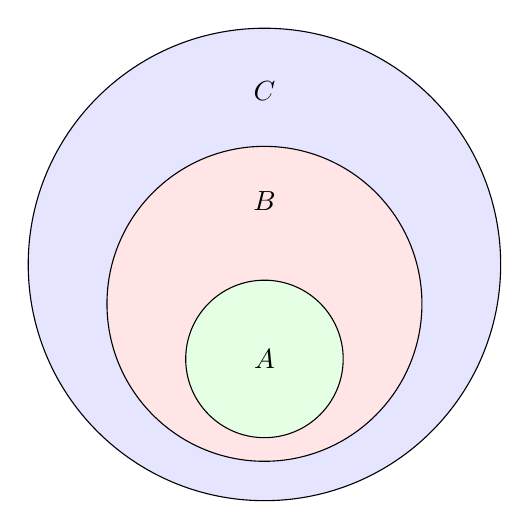
\begin{tikzpicture}
    \draw[fill=blue!10] (0,0) circle (3cm);
    \node at (0, 2.2) {$C$};
    \draw[fill=red!10] (0,-0.5) circle (2cm);
    \node at (0, 0.8) {$B$};
    \draw[fill=green!10] (0,-1.2) circle (1cm);
    \node at (0, -1.2) {$A$};
\end{tikzpicture}
\end{center}
\end{proof}

\subsection*{Solution 17}
\begin{proof}
We proceed by evaluating the truth set of the precondition $P(x)$. By the positive-definite axiom of Euclidean norm spaces, for any vector $v \in \mathbb{R}^d$, $\|v\|^2 \ge 0$. Therefore, for any $x, \mu, \nu \in \mathbb{R}^d$:
\[ \|x - \mu\|^2 \ge 0 \quad \text{and} \quad \|x - \nu\|^2 \ge 0 \]
The sum of two non-negative real numbers must be non-negative:
\[ \|x - \mu\|^2 + \|x - \nu\|^2 \ge 0 \]
The trigger condition $P(x) < 0$ is logically impossible. The set of states triggering the fallback protocol is $S = \{x \in \mathbb{R}^d : P(x) \text{ is true}\} = \emptyset$. By Kolmogorov's first axiom of probability, the measure of the empty set is exactly zero. Thus, the probability measure of triggering the fallback is $\mathbb{P}(Q(X)) = \mathbb{P}(\emptyset) = 0$.
\end{proof}

\subsection*{Solution 18}
\begin{proof}
We proceed via a vacuous proof. Let $P(\omega)$ be the statement ``strategy $\omega$ yields a risk-free profit with zero initial investment''. By the fundamental definition of an arbitrage-free market, no such arbitrage strategy can exist. Therefore, the statement $P(\omega)$ is strictly false for all possible trading strategies $\omega \in \Omega$. Because the premise of the implication is invariably false, the implication $P(\omega) \implies Q(\omega)$ (where $Q(\omega)$ is the conclusion ``$\omega$ guarantees a risk-free loss'') evaluates to true vacuously.
\end{proof}

\subsection*{Solution 19}
\begin{proof}
The structural flaw in the proof is \textbf{Domain Blending} (specifically, misapplying real number axioms to the complex domain). The proof relies on the assertion that ``the square of any number is non-negative'', which is an axiom strictly bounded to $\mathbb{R}$ ($\forall x \in \mathbb{R}, x^2 \ge 0$). 
In the complex plane $\mathbb{C}$, this axiom fails. For example, let $x = i \in \mathbb{C}$. Then $x^2 = i^2 = -1$. Since $-1 < 0$, the hypothesis $x^2 < 0$ is \textit{not} impossible in $\mathbb{C}$. Therefore, the hypothesis is not always false, and claiming the implication is vacuously true is a logical fallacy. 
(Note: The theorem itself is actually true via a direct proof: if $x^2 < 0$, then $x = bi$ for some $b \in \mathbb{R} \setminus \{0\}$. Then $x^4 = (bi)^4 = b^4 i^4 = b^4(1) > 0$. However, the provided vacuous proof is entirely invalid).
\end{proof}

\subsection*{Solution 20}
\begin{proof}
We proceed via a direct proof. Assume $x, y \in \mathbb{Q}$. By the definition of rational numbers, there exist integers $a, b, c, d \in \mathbb{Z}$ with $b \neq 0$ and $d \neq 0$ such that $x = \frac{a}{b}$ and $y = \frac{c}{d}$. We first factor the algebraic expression:
\[ x^2 + 2xy + y^2 = (x + y)^2 \]
Substituting the rational definitions into the factored form:
\[ \left(\frac{a}{b} + \frac{c}{d}\right)^2 = \left(\frac{ad + bc}{bd}\right)^2 = \frac{(ad + bc)^2}{(bd)^2} \]
Let $p = (ad + bc)^2$ and $q = (bd)^2$. Since the integers are closed under addition and multiplication, $p, q \in \mathbb{Z}$. Since $b \neq 0$ and $d \neq 0$, the Zero Product Property ensures $q = b^2 d^2 \neq 0$. Thus, the expression equals $\frac{p}{q}$, which satisfies the definition of a rational number.
\end{proof}

\subsection*{Solution 21}
\begin{proof}
We proceed via a vacuous proof. The domain is $\mathbb{N}$, meaning $n \ge 1$. Because $n > 0$, we can multiply both sides of the hypothesis inequality $n + \frac{1}{n} < 2$ by $n$ without reversing the inequality sign:
\[ n^2 + 1 < 2n \]
Subtracting $2n$ from both sides yields:
\[ n^2 - 2n + 1 < 0 \]
Factoring the perfect square gives:
\[ (n - 1)^2 < 0 \]
By the axioms of real numbers, the square of any real number (and thus any natural number) is non-negative, meaning $(n - 1)^2 \ge 0$. The inequality $(n - 1)^2 < 0$ is a logical contradiction. Because the hypothesis is false for all $n \in \mathbb{N}$, the implication is vacuously true.
\end{proof}

\subsection*{Solution 22}
\begin{proof}
We establish the logical equivalence of an implication and its contrapositive using propositional logic. We expand the left-hand statement using Material Implication:
\[ P \implies Q \equiv \neg P \lor Q \]
Next, we expand the right-hand statement (the contrapositive) using Material Implication:
\[ \neg Q \implies \neg P \equiv \neg(\neg Q) \lor \neg P \]
Applying Double Negation elimination ($\neg(\neg Q) \equiv Q$):
\[ \equiv Q \lor \neg P \]
By the Commutative Law of logical disjunction ($A \lor B \equiv B \lor A$):
\[ \equiv \neg P \lor Q \]
Since both statements reduce to $\neg P \lor Q$, they are logically equivalent.
\end{proof}

\subsection*{Solution 23}
\begin{proof}
To find a counterexample, we must find a real number $x \in \mathbb{R}$ such that the hypothesis ($x^3 > 0$) is true, but the conclusion ($x > 1$) is false. 
Let $x = 0.5$. 
We evaluate the hypothesis:
\[ (0.5)^3 = 0.125 > 0 \]
The hypothesis evaluates to true. 
We evaluate the conclusion:
\[ 0.5 > 1 \]
The conclusion evaluates to false. Because the premise is true and the conclusion is false, the implication is false. This serves as a valid counterexample.
\end{proof}

\subsection*{Solution 24}
\begin{proof}
We proceed via a direct proof. Assume $a$ and $b$ are odd integers. By definition, there exist integers $k, m \in \mathbb{Z}$ such that $a = 2k + 1$ and $b = 2m + 1$. We evaluate their product:
\begin{align*}
    ab &= (2k + 1)(2m + 1) \\
       &= 4km + 2k + 2m + 1
\end{align*}
To show this is an odd integer, we factor out a $2$ from the first three terms:
\[ ab = 2(2km + k + m) + 1 \]
Let $j = 2km + k + m$. Since the integers are closed under multiplication and addition, $j \in \mathbb{Z}$. We have expressed $ab$ as $2j + 1$ for an integer $j$. By definition, $ab$ is an odd integer.
\end{proof}

\subsection*{Solution 25}
\begin{proof}
We proceed via a vacuous proof. Let $P(x)$ be the hypothesis $4x^2 - 4x + 2 \le 0$. We complete the square for the quadratic expression:
\[ 4x^2 - 4x + 2 = (4x^2 - 4x + 1) + 1 = (2x - 1)^2 + 1 \]
By the properties of real numbers, $(2x - 1)^2 \ge 0$ for all $x \in \mathbb{R}$. Adding $1$ to both sides yields:
\[ (2x - 1)^2 + 1 \ge 1 > 0 \]
Thus, the statement $(2x - 1)^2 + 1 \le 0$ is logically impossible. Because the hypothesis is false for all $x \in \mathbb{R}$, the implication is vacuously true.
\end{proof}

\subsection*{Solution 26}
\begin{proof}
We analyze the inequality defining the event space $A$:
\[ X(\omega)^2 + Y(\omega)^2 < 2X(\omega)Y(\omega) \]
Subtracting $2X(\omega)Y(\omega)$ from both sides yields:
\[ X(\omega)^2 - 2X(\omega)Y(\omega) + Y(\omega)^2 < 0 \]
Factoring the perfect square gives:
\[ (X(\omega) - Y(\omega))^2 < 0 \]
By the axioms of real numbers, the square of any real quantity is non-negative. Thus, the condition $(X(\omega) - Y(\omega))^2 < 0$ is impossible for any outcome $\omega \in \Omega$. The event set is therefore the empty set: $A = \emptyset$. By Kolmogorov's axioms of probability, the measure of the empty set is zero. Thus, $\mathbb{P}(A) = 0$.

\begin{center}
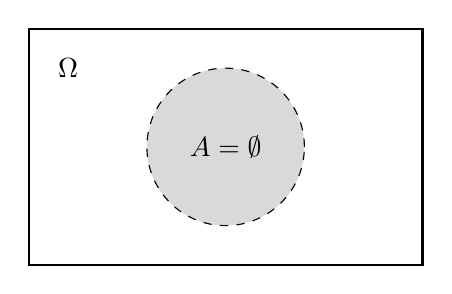
\begin{tikzpicture}
    \draw[thick] (0,0) rectangle (5,3);
    \node at (0.5, 2.5) {$\Omega$};
    \draw[fill=gray!30, dashed] (2.5,1.5) circle (1cm);
    \node at (2.5,1.5) {$A = \emptyset$};
\end{tikzpicture}
\end{center}
\end{proof}

\subsection*{Solution 27}
\begin{proof}
We proceed via a vacuous proof. Let $P(x)$ be the hypothesis $2x = x^2 + 2$. Rearranging the equation by moving all terms to one side yields:
\[ x^2 - 2x + 2 = 0 \]
We complete the square:
\[ (x^2 - 2x + 1) + 1 = 0 \implies (x - 1)^2 + 1 = 0 \implies (x - 1)^2 = -1 \]
Since $x \in \mathbb{Z} \subset \mathbb{R}$, the square of $(x-1)$ must be non-negative, meaning $(x-1)^2 \ge 0$. It is mathematically impossible for a non-negative number to equal $-1$. Thus, there are no integer solutions to the hypothesis equation. Because the hypothesis is false for all $x \in \mathbb{Z}$, the implication is vacuously true.
\end{proof}

\subsection*{Solution 28}
\begin{proof}
The structural flaw in the proof is \textbf{Variable Aliasing}. The proof defines $x = 2k+1$ and $y = 2k+1$, utilizing the exact same dummy variable $k$ for both integers. This implicitly forces the assumption that $x = y$, which is not stated in the theorem (the theorem applies to \textit{any} two odd integers, such as $x=7$ and $y=3$). 
To correct this, one must use distinct variables. Let $x = 2k+1$ and $y = 2m+1$ for $k, m \in \mathbb{Z}$. Then $x - y = (2k+1) - (2m+1) = 2(k - m)$. This valid derivation only proves that the difference is an even integer, not necessarily a multiple of $4$. (Indeed, $7 - 3 = 4$ is a multiple of $4$, but $7 - 5 = 2$ is not, proving the original theorem is actually false).
\end{proof}

\subsection*{Solution 29}
\begin{proof}
To find a counterexample, we must define sets $A, B, C$ such that the hypothesis ($A \subseteq B \cup C$) is true, but the conclusion ($A \subseteq B \lor A \subseteq C$) is false. 
Let $A = \{1, 2\}$, $B = \{1\}$, and $C = \{2\}$. 
We evaluate the hypothesis:
\[ B \cup C = \{1\} \cup \{2\} = \{1, 2\} \]
Since $A = \{1, 2\}$, the statement $A \subseteq B \cup C$ is true. 
We evaluate the conclusion:
$A \subseteq B$ is false because $2 \in A$ but $2 \notin B$. 
$A \subseteq C$ is false because $1 \in A$ but $1 \notin C$. 
Since both parts of the disjunction are false, the conclusion is false. This provides a valid counterexample.
\end{proof}

\subsection*{Solution 30}
\begin{proof}
We proceed via a direct proof. Assume $A \cap B = A \cup B$. To prove set equality $A = B$, we must demonstrate mutual inclusion: $A \subseteq B$ and $B \subseteq A$.
\newline\newline
\textbf{Part 1 ($A \subseteq B$):} Let $x \in A$. By the definition of a set union, $x \in A \cup B$. Because we assumed $A \cup B = A \cap B$, it follows by substitution that $x \in A \cap B$. By the definition of a set intersection, $x \in A \cap B \implies x \in B$. Thus, we have shown $x \in A \implies x \in B$, meaning $A \subseteq B$.
\newline\newline
\textbf{Part 2 ($B \subseteq A$):} Let $y \in B$. By the definition of a set union, $y \in A \cup B$. Because we assumed $A \cup B = A \cap B$, it follows by substitution that $y \in A \cap B$. By the definition of a set intersection, $y \in A \cap B \implies y \in A$. Thus, we have shown $y \in B \implies y \in A$, meaning $B \subseteq A$.
\newline\newline
Since we have rigorously established both $A \subseteq B$ and $B \subseteq A$, it follows by the axiom of extensionality that $A = B$.
\end{proof}

\newpage

\section{Concept Checklist \& Question Mapping (Reference)}
\label{sec:checklist_end}
\begin{itemize}
    \item \textbf{Trivial Proof (Continuous Domain):} Problem 3
    \item \textbf{Vacuous Proof (Continuous Domain):} Problems 1, 7, 11, 25
    \item \textbf{Vacuous Proof (Discrete Domain):} Problems 2, 15, 21, 27
    \item \textbf{Direct Proof (Parity of Integers):} Problems 4, 10, 24
    \item \textbf{Direct Proof (Divisibility):} Problems 5, 12
    \item \textbf{Direct Proof (Rational Numbers):} Problems 6, 20
    \item \textbf{Algebraic Manipulations (Completing the Square):} Problems 1, 3, 25, 27
    \item \textbf{Algebraic Manipulations (Cyclic Symmetry):} Problem 7
    \item \textbf{Domain Boundary Conditions:} Problems 2, 21
    \item \textbf{Logical Equivalences:} Problems 8, 13, 22
    \item \textbf{Counterexamples:} Problems 9, 14, 23, 29
    \item \textbf{Fallacy Identification (Misapplying Axioms):} Problem 19
    \item \textbf{Fallacy Identification (Variable Aliasing):} Problem 28
    \item \textbf{Abstract Real-World Modeling (AI Constraint Sets):} Problem 17
    \item \textbf{Abstract Real-World Modeling (Quant Finance):} Problem 18
    \item \textbf{Abstract Real-World Modeling (Measure-Theoretic Probability):} Problem 26
    \item \textbf{Set Theory (Subset Inclusion \& Equality):} Problems 16, 29, 30
\end{itemize}

\end{document}